\chapter{Hardware and Embedded Software}
\label{cha:hardware}

\section{User Interface}
As most of the user interface capabilities should be included in the Android application software, the transducer hardware can be designed to include only very basic user interface elements.

\paragraph{Input}
As the system should include the possibility to trigger measurements pushing a hardware button on the transducer device (rather than unlocking the Android device, starting the app and triggering the measurement there), a single button is needed which needs to be wired to an Arduino input able to trigger an interrupt. The pin is configured as as an input with the pull-up resistor enabled. The button connects the pin to ground while it is pushed; an interrupt accordingly is triggered on a falling edge of the pin input signal.

\paragraph{Signaling}
In order to let the user know if the device is ready for operation, it includes three LEDs that show the status of different system components:

\paragraph{Sending Indicator}
This LED has two use cases. It should light up when the user triggers a measurement and turn off when the Android device acknowledged having received the data. This means it gives a fast response to users showing their button press was received and it signals the time needed to handle the button press. The time needed to collect the sensor data might be significant and thus the user is informed that he should not trigger another measurement while the previous one is not completed. If the LED does not turn off, it indicates a connection fault and the user might need to address this by connecting the Android devece.

\paragraph{Bluetooth Status}
The bluetooth status LED should show the connection state of the bluetooth module. As most bluetooth modules do not directly transmit the connection state to the Arduino, the LED should be connected directly to the bluetooth module and relay the signalling normally shown by the internal status LED. Most modules contain a state pin to get this signal. If there is no possibility to get this signal, the LED might be left out.

\paragraph{GPS Status}
The GPS status can be derived either from the GPS module directly or queried in the embedded software. As the embedded software is closer to the transducer output, the state is determined in the embedded software and thus the LED is connected to an Arduino output pin (note that some Arduinos including the Arduino Due can only drive small currents and an appropriate current limiting resistor must be used).

\section{Hardware Requirements}
In general, it should be possible to build the sensor transducer hardware based on any Arduino. The setup must include a Bluetooth serial pass-through module. 

\section{Hardware Selection}
As the complexity of the project might significantly increase when a multitude of different hardware components must be supported, this section defines the requirements applied to the hardware and proposes suitable common components which are also used for the demonstration assembly.

\subsection{Bluetooth Module}
As defined in the previous chapter, the communication between the transducer hardware and the Android device should use the Bluetooth radio frequency communication (RFCOMM) profile. Any module that is able to pass serial data received via a TTL connection through to a Bluetooth RFCOMM channel should work for this purpose. In order to avoid damages to the hardware, the module either needs to use the same voltage as the Arduino or voltage limiting circuitry needs to be included. 

The proposed module is the HC-05 on a ZS-040 (see \cite{HC-05}) carrier board. This combination is commonly available and can typically be manually reprogrammed using AT-commands. Most of the carrier boards include a state pin which can be connected to the status LED. The only alternative commonly found is the HC-06 module which for this use case does exactly the same as the HC-05 module (while it does not support working as a Bluetooth master).

\subsection{GPS module}
As most GPS modules commonly available for discrete electronic circuits are using standardized NMEA-sentences to transmit the received data, these modules can be used interchangeably. The embedded software designed for this project exclusively supports GPS-receivers transmitting their data encoded as NMEA-Sentences via a serial (TTL) connection.

The module used in the demonstration device is an Adafruit Ultimate GPS (see \cite{AdaUltGPS}) module as it provides some useful additional features by allowing an external antenna to be connected via a $\mu$FL-connector and including an enable pin which can be used to disable the module. 

\section{Sensor Hardware Compatibility}
The Arduino platform is well known for its wide sensor compatibility. Typically, a library providing some kind of abstraction from the actual sensor interface is used and can easily be deployed to adapt the code for new sensors. 

Most Arduino boards provide the following interfaces for sensors:
\begin{itemize}
	\item UART (serial communications)
	\item I$^2$C (Inter Integrated Circuit, also called Two Wire Interface or TWI)
	\item Analog voltage input (10 or 12-bit resolution)
	\item Digital IO (used e.g. for the one-wire-bus)
	\item SPI (Serial Peripheral Interface Bus)
\end{itemize}

All of these interfaces can be used to connect sensors and other data sources. The software system is intended to be used with sensors that produce real (i.e. floating point) numbers as measurement output. The main design goal is support for one-shot readout, but sensors regularly producing data and sending it to the Arduino might as well be used.

Some Arduino models support additional interfaces such as CAN (Controller Area Network), Bluetooth, Sigfox (a low-power, long range wireless network technology) or GSM (standard cellular networks). These interfaces might be used according to their availability on the hardware platform chosen. 

If a sensor not directly compatible with the chosen hardware platform should be used, often converter modules can be used to transduce the data to a compatible interface. Common examples are high-resolution analog-digital converters connected to the I$^2$C-bus or CAN-Modules connected to the Arduino SPI bus.

\section{Circuit Wiring}
\subsection{Power Supply}
As the module should be usable everywhere, it cannot rely on mains power and therefore needs an independent power source. While powering the module from the Android device might be an option on some Android devices (which support on-the-go power via USB and contain an appropriate voltage regulator), doing so would neither be possible in general nor practical as it would quickly discharge the device battery. Therefore an independent battery should be used. All Arduino boards contain linear voltage regulators that can be used to regulate feed voltages that typically need to be around 0.3 Volt above the required device voltage. A 3.3 V Arduino can therefore be operated from any voltage above 3.6 V DC and a 5 V model typically needs 5.3 V (6 V is recommended) to be fed to the linear regulator. On 3.3 V boards this allows the system to be operated from a single LiIon-Cell or at least three NiMH or Alkaline batteries. As Lithium Batteries require extra components to be charged and to prevent deep discharges or short-circuits, the proposed device should be operated from NiMH rechargeable or alkaline primary battery cells. These cells can be exchanged by the user and in case of NiMH rechargable cells be recharged using standard chargers. Using alkaline primary batteries allows the device to be used with widely available batteries bought from a store in case no charging facilities are avaliable. The recommended size is AA (mignon), as this size provides a reasonable runtime for the device. Even though using only three cells might provide a sufficient voltage, using four cells is recommended for 3.3 V devices as the cells voltage will drop during discharge and on energy usage peaks. Using four cells allows the cells to be discharged to a typical end-point voltage of 0.9 V per cell instead of 1.2 V if only three cells are used.

\subsection{General considerations}
As the device should be as easy as possible to build, it should be possible to build the transducer module without soldering. As many sensors are available as modules that can be plugged into a breadboard or connected using jumper cables, it is recommended to use this kind of sensors. The wiring can then be made on a breadboard and using jumper wires which in turn makes the assembly modifiable and the modules reusable for other purposes when the transducer is not needed anymore.

Using a 3.3 V Arduino Pro Mini as an example, the basic circuit wiring is shown in figure \ref{fig:pro-mini-diagram} and a visual representation of the assembly on a breadboard is shown in figure \ref{fig:pro-mini-diagram}. Using other Arduino modules typically requires the Arduino to not be directly plugged into the breadboard but connected using jumper wires instead.

\begin{figure*}[t]
\centering
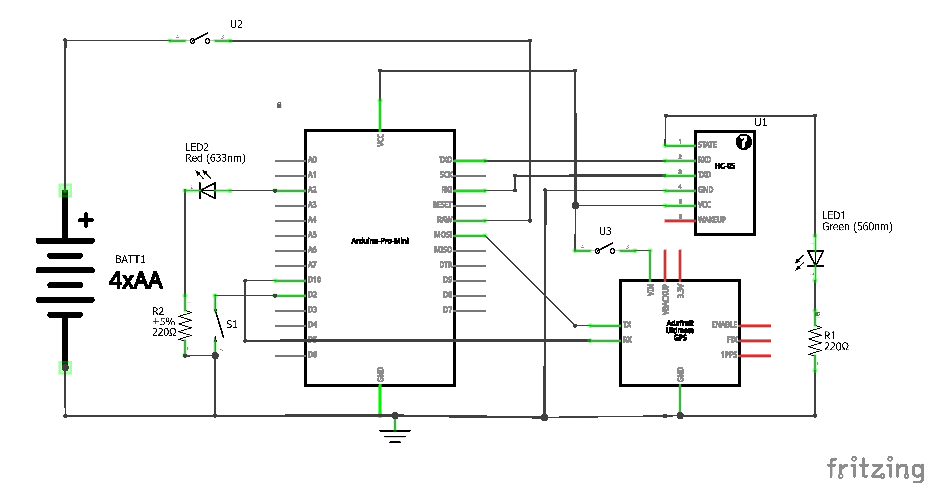
\includegraphics[width=1.0\textwidth]{src/pro_mini_diagram.pdf}
\caption{Proposed circuit for the basic transducer parts}
\label{fig:pro-mini-diagram}
\end{figure*}

\begin{figure*}[t]
\centering
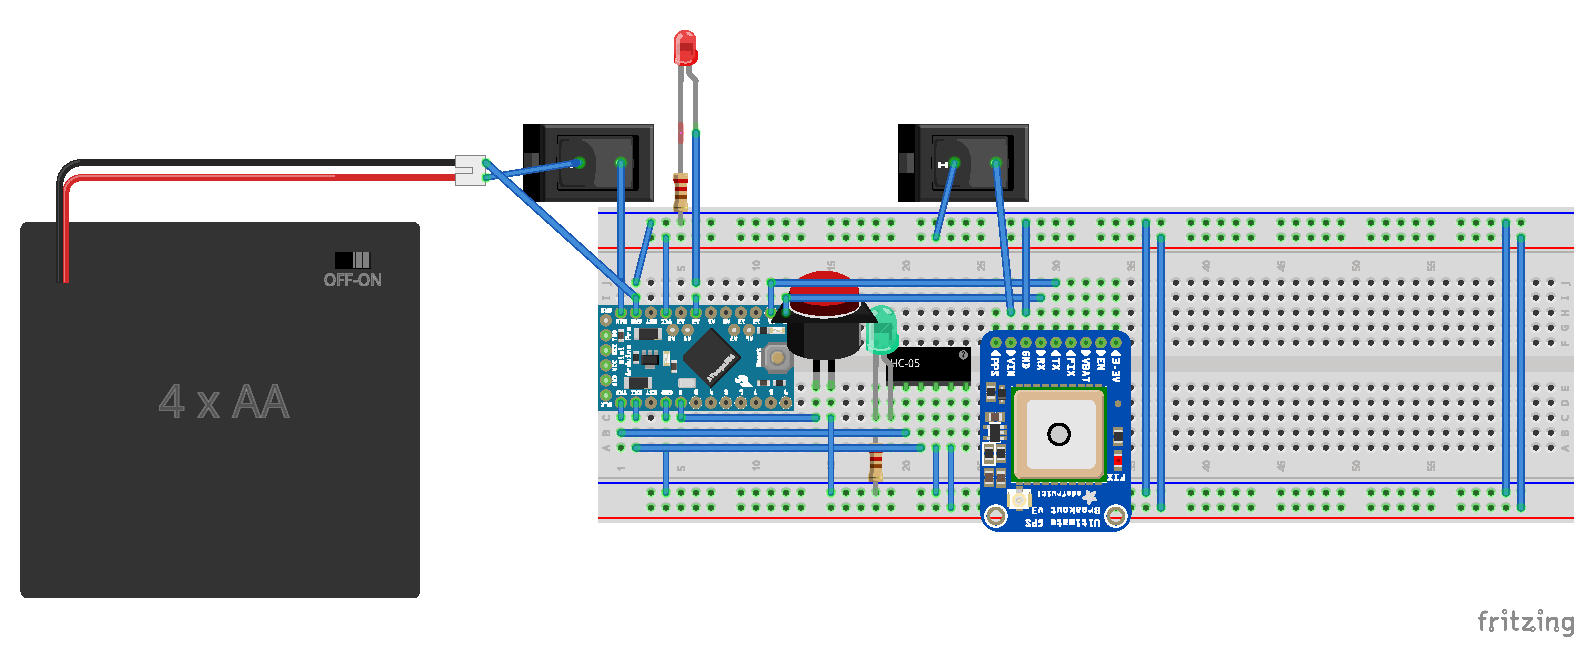
\includegraphics[width=1.0\textwidth]{src/pro_mini_breadboard.pdf}
\caption{Breadboard wiring example for the basic transducer parts}
\label{fig:pro-mini-breadboard}
\end{figure*}

\subsection{Demonstration Assembly}
The demonstration assembly is the version of the transducer device used for performance and energy-usage testing. It uses a 3.3 V Arduino Pro Mini module, the HC-05 Bluetooth Module and an Adafruit Ultimate GPS Module connected to an active external antenna. The power is supplied by four AA-size NiMH rechargeable batteries. The assembly follows the circuit wiring proposed in the previous section.

In order to test the system using actual sensors, a DHT11 air humidity and temperature sensor and an encapsulated DS18B20 digital temperature sensor are connected to the Arduino module. This sensors have a low energy consumption and will be included in all system performance tests.

\subsection{Case}
As the electronic components need to be protected from mechanical forces and accidental short circuits, a case for the demonstration assembly has been made using a 3D printer. The case was designed using Autodesk Fusion 360 (see \cite{f360}). The case was specifically designed to include the user interface elements used in the demonstration assembly. Design files for the base element and the top part can are included in the appendix. 

\begin{figure*}[h]
\centering
\includegraphics[width=1.0\textwidth]{src/demonstration_device.jpg}
\caption{The demonstration device enclosed in its case. On the left side, the cable connecting the external temperature sensor exits the case.}
\label{fig:demonstration_device}
\end{figure*}

\section{Energy Consumption Optimization}
As the system should be able to run on battery power, a long runtime before the batteries need to be changed is desirable. Therefore, the following proposed optimizations have been reviewed.

\subsection{Bluetooth Low-Energy}
The Bluetooth low energy standard was designed to allow significantly reduced energy consumption when compared to classic Bluetooth. As manufacturers of electronic modules for Arduino often do not publish information on energy consumption of their modules, the effects need to be measured in real testing devices. A Hameg Instruments HM8134 laboratory power supply has been used to measure the power consumption of the HC-05 Bluetooth module proposed for the transducer and a pin-compatible HM-10 Bluetooth low energy module. Both modules are specified to be used with a 3.3 V (dc) 50 mA power supply. The modules contain a low-dropout voltage regulator and can therefore be fed using higher voltages, however in this experiment, both modules are fed using 3.3 V and stabilized using a 1000 $\mu F$ capacitor next to the power input pins of the modules.

The modules differ significantly in their energy usage patterns. The HM-10 Bluetooth low energy module has a virtually constant current draw of around 9 mA. Opposed to that, the HC-05 module uses different currents depending on the connection state. While the module is searching, the current draw is around 40 mA, when connected and idle the module draws between 2 and 4 mA. When a message is sent, the current peaks to about 20 mA and stays around 15 mA for about 5 seconds. As the connection should be in the connected idle state for most of the time, the energy usage using the HC-05 Bluetooth module is significantly lower than using the HM-10 Bluetooth low energy module in most use cases. Therefore, it was decided to not include the option to use this Bluetooth low energy module in the system.

The average current values when run at 3.3 V supply voltage recorded during the measurements are the following:
\begin{center}
  \begin{tabular}{ | c | c |}
    \hline
	\hline
    HC-05 Bluetooth module (connected) & 2.38 mA \\ \hline
    HC-05 Bluetooth module (searching) & 39.91 mA \\ \hline
    HM-10 Bluetooth LE module (connected) & 10 mA \\ \hline
    HM-10 Bluetooth LE module (searching) & 8.88 mA \\ \hline
    \hline
  \end{tabular}
\end{center}

\subsection{Interrupt-Driven Programming}
Microprocessors typically include means to enter power saving states while only a limited subset of the processors capabilities are needed. While a microprocessor is waiting for user input it can often be put into a sleep state that includes the capability to wake up the processor when an external interrupt occurs. However, the Arduino software platform proposes the use of so-called busy loops to implement software features. As the energy usage of the complete Arduino module can be measured to be 5 mA using the same method as for the Bluetooth modules, the cost of breaking the Arduino programming paradigm in order to reduce the energy usage is considered unreasonable. Furthermore, the way GPS data is received on devices having only a single hardware serial transceiver imposes further problems when an interrupt driven programming model should be used as a software serial connection can only be used while the microprocessor is completely awake.

\subsection{Low-Voltage Circuit Components}
The components used in the demonstration assembly have been selected to be powered using 3.3 V. Most modern microelectronic components are available in a 3.3 V version while there are only few components to be found that might run on lower voltages. As Arduino modules typically contain a low dropout linear voltage regulator, this means the minimum input voltage for a system containing only 3.3 V compatible parts is around 3.6 V and therefore fewer battery cells are needed to power the system compared to a system using components running at 5 V. 

\subsection{Switching Power Supply}
Most Arduino boards (including the one used in the demonstration assembly) contain a low-dropout linear voltage regulator it can be fed with input voltages between 3.6 and around 7.5 V (the upper limit is determined by heat dissipation). The electronic parts can however be fed directly when a sufficiently stabilized input voltage is available. As linear voltage regulators maintain the current while the voltage at the output is reduces compared to the input, they offer a low efficiency when the voltage difference between input and output is high. Switching voltage regulators might have a higher efficiency in some use cases.

Using a the demonstration device as an example, a test on possible efficiency gains has been carried out using a TSRN 1-2433 switching voltage regulator produced by TRACO. Even though the switching supply reduces energy usage on high input voltages, the effects of using this module in conjunction with the 4 NiMH cell power source are supposed to be negative. This switching voltage regulator has a minimum input voltage of 4.6 V and can therefore not use the whole energy stored in the cells as they cannot be discharged much below the nominal voltage of 1.2 V per cell. Even though the switching regulator offers a minor advantage in conversion efficiency, the overall runtime using a set of four NiMH rechargeable cells is therefore supposed to be lower when this switching module is used.

For higher input voltages (like 12 V from a lead battery) using a switching regulator however might be a considerable advantage. The linear regulator on the Arduinoboard might even overheat when a high current is drawn while a high supply voltage is used. The total average power consumption at different input voltages is shown in figure \ref{fig:switching_linear}.

\begin{figure*}[ht]
\centering
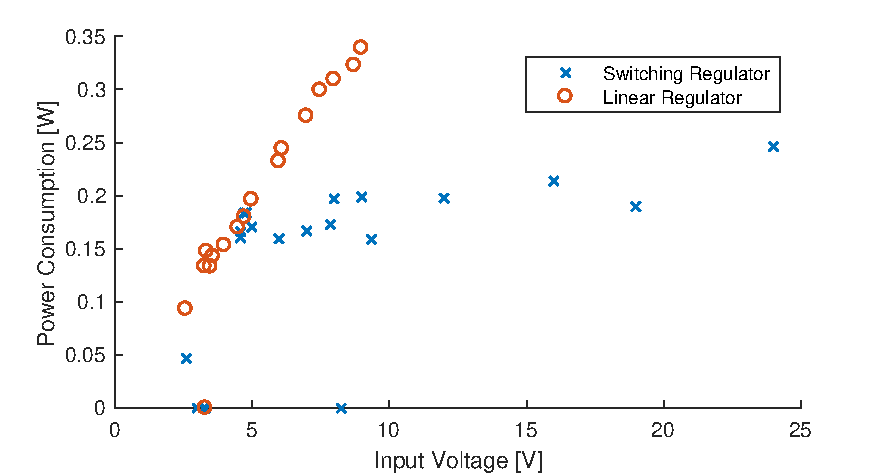
\includegraphics[width=1.0\textwidth]{src/switching_linear.pdf}
\caption{Comparison of the energy consumption between the linear regulator on the Arduino Pro Mini board and an external switching regulator}
\label{fig:switching_linear}
\end{figure*}

\section{Embedded Software}
The embedded software used on the transducer hardware was developed in the Arduino-specific C++ dialect. It was developed in using the visual micro (see \cite{vMicro}) plugin for Microsoft Visual Studio, but it can also be modified and built using the official Arduino IDE. 

The software is divided in two parts, the first one needs to be modified by users adapting the system to their needs while the second one is the technical basis that normally does not need to be modified. The code used for the demonstration device is included in the appendix of this document.

\subsection{Library Usage}
\subsubsection{GPS}
Most GPS-modules able to interface with Arduino software will do so transmitting so-called NMEA sentences (see \cite{NMEASentences}) via a serial interface. As this text-based format needs to be parsed into a format usable for retransmission of the relevant data portion there needs to be either a considerable amount of parser code included in the software or an external library used. As code readability, reusability and standard conformity can be significantly improved by using a library, it was decided a library should be used for the NMEA sentence parsing.

\paragraph{Adafruit GPS}
The Adafruit GPS Library (see \cite{AdaUltGPS}) is a library provided to be used with the Adafruit GPS module used in the demonstration assembly. There are however no official statements on compatibility with other GPS receivers and therefore this library is not considered to be a general solution for arbitrary GPS devices. 

\paragraph{TinyGPS}
TinyGPS (see \cite{TinyGPS} is a commonly used library for parsing NMEA sentences on the Arduino platform. It was written by Mikal Hart and is considered to be a good library for very restricted hardware environments.

\paragraph{TinyGPS++}
The TinyGPS++ (see \cite{TinyGpsPlus}) library is a spiritual successor of the TinyGPS library containing an enhanced set of features. The author recommends using it instead of TinyGPS in environments having enough resources to handle it. As program size is not a major concern for this embedded software, this library is used.

\subsubsection{Communications}
As a Bluetooth RFCOMM channel is used for communication towards the Android device, the microcontroller must interface with the Bluetooth module. This project uses transparent serial-pass-through Bluetooth modules and therefore there is no need for any interface library apart from the UART hardware interface code included in the Arduino core libraries.

\subsubsection{Data formatting}
The protocol specification (see \ref{sec:protocol}) stipulates the use of of the JavaScript Object Notation (JSON) as data transmission format for the serial communication towards the Android device. There is only one well-known Arduino library for JSON encoding which is called ArduinoJson (see \cite{ArduinoJson}) (the aJson library (see \cite{aJson}) cannot be considered an adequate alternative as it will not work on ATMega168-based boards). The library has a reasonably low memory footprint and allows for the creation of JSON Objects as proposed by the protocol specification.

\subsubsection{Sensors}
As the system specification allows for manifold sensor types and interfaces, normally some libraries should be used to collect the sensor data.

\paragraph{Demonstration Assembly}
\label{p:demonstration_device}
As the demonstration assembly contains two different sensor types, two libraries are used for sensor readout. The sensors are part of a proof of concept (as opposed to the main system components) and therefore the librarys used were chosen as first-that-fits. The libraries used are the \texttt{DHT Temperature \& Humidity Unified Sensor Library} (see \cite{DHTlib}) for the DHT11 temperature and humidity sensor and the OneWire (see \cite{OW}) and the DallasTemperature library (see \cite{DallasTemp}) for the DS18B20 One Wire temperature sensor.

\subsection{Basic Functionality}
In chapter (\ref{cha:requirements}) the basic requirements for the transducer device are outlined to be reading out sensors and sending it to the Android application.

\subsection{Sensor Readout}
The sensor readout needs to be adjusted to the type of sensor incorporated in the system actually build. Examples for sensor readout code can be found online for most common sensor models. The software especially focusses on sensors that allow one-shot readout, but code might be incorporated to support other readout mechanisms.

\subsubsection{One-Shot readout}
All code reading out the connected sensors and putting it in the JSON structure described in the protocol specification can be found in a single function that is called when the trigger button has been pushed or a measurement has been triggered through the Android application.

\subsection{GPS positioning}
The GPS receiver connection in the system might basically have three different states which must be handled accordingly.

\paragraph{No GPS Receiver or disabled}
If there is no GPS receiver included in the transducer hardware or the GPS receiver is disabled (which is a feature that might be implemented as a hardware switch or compiled into the software), there should be no position object included in the transmission data or the position object should only contain the isValid key. If the GPS feature is disabled during software compilation, the JSON message generated by the transducer should not contain a position object.

\paragraph{Waiting for GPS fix}
Normally a user should wait for the GPS position to be fixed before they trigger a measurement. If a measurement is triggered anyway, a position object containing only the isValid key should be sent to the Android device.

\paragraph{Position fixed}
When the position is fixed (and the age does not exceed a threshold of 15 seconds), a full position object containing the location information is included in the sentence.

\subsection{Additional Features}
\subsubsection{User Interface}
Apart from an LED that can be directly connected to the Bluetooth module to show its connection status, the software contains means to drive two status LEDs showing the GPS state and the state of a currently ongoing measurement. The GPS LED blinks while the device is on and there is no position fix and shows continuous light while a position not older than three seconds is available. The state LED for the current measurement is turned on when a measurement is triggered and turned off when an acknowledgement has been received.

\subsubsection{Resending Information}
\label{subsubs:resending}
\paragraph{Data Retention Mechanism}
The microcontrollers used in the Arduino Platform usually contain three different types of memory: SRAM, Flash and EEPROM. Normally the SRAM is used to store the data while it is processed and sent. However, the main downside of using SRAM is data loss in case of power loss or hardware resets. As both other memory types are non-volatile and thus retain their data also in case of a power loss, they are better suited for data retention purposes. The Arduino platform favors the use of the EEPROM memory by providing libraries and documentation. As also the lifecycle specified for the EEPROM is much longer, it is used for data retention in this project. The mechanism as implemented cannot be used on Arduino boards not equipped with an EEPROM like the Arduino Due. For these Boards, another mechanism based on a string buffer located in the SRAM has been developed. As SRAM is a volatile memory, the SRAM buffer cannot hold the data through power losses.

\subparagraph{Product Lifecycle Considerations}
As EEPROM allows only a limited number of write cycles, the overall product lifecycle must be considered when using EEPROM. A typical example lifespan of for the EEPROM included in an Arduino is the one from the ATmega328 (see \cite{ATmega328}) used in the demonstration device. It has a specified minimum lifecycle of 100 000 write cycles (after that often the data retention time will fade). A minimum lifecycle of 100 000 measurements is considered sufficient for the use cases proposed in this project.

\subsection{Performance Considerations}
When large libraries are used to handle the sensor data or there are many sensors connected, the SRAM space on the Arduino might be too small. In order to reduce problems that might arise from this, all constant strings in the code are encapsulated using the F()-Macro, which reads the strings from the program flash memory instead of transferring it into SRAM on startup.

\subsection{Fault Behavior}
Hardware and transmission faults might occur for unforeseen reasons and therefore the device should be able to handle these gracefully. This section covers the most common problems that might occur during operation.

\subsubsection{GPS Receiver}
As the GPS receiver might need a significant amount of time (about 30 seconds when there is no buffer battery) for the first position fix (or the fix is impossible due to obstacles blocking the signal), there is a significant period of time in which the device does not have valid location information. If a GPS status LED is incorporated, the user can wait until a position fix occurs or rely on the Android device to deliver location information. On the protocol side, a message is sent that contains a position object which only contains the isValid key and a false value. 

\subsubsection{Bluetooth}
Different Bluetooth modules might exhibit different behaviour regarding state pins exposed to the outside. Typically, the user can see a status LED showing the connection state in some way. If a measurement is triggered while there is no connection, the data is repeatedly resend (see \ref{subsubs:resending}) until an acknowledge is received from the Android device. If a new measurement is triggered before the data is acknowledged (shown by the state LED), the previous measurement might be lost.

\subsection{Extensibility}
Only standard Arduino hardware and software parts are used in this project, all extensibility options available for the Arduino platform might be incorporated into this system. This includes the use of software libraries, modules, shields and other electronic components.

